\chapter{Lab 10 - Final Project}

%%%%%%%%%%%%%%%%%%%%%%%%%%%%%%%%%%%%%%%%%%%%%%%%%%%%%%%%%%%%%%%%%%%%%%%%%%%%%%%%%%%%%%%%%%%%%%%%%%%%%%%
\section{Objective}
%%%%%%%%%%%%%%%%%%%%%%%%%%%%%%%%%%%%%%%%%%%%%%%%%%%%%%%%%%%%%%%%%%%%%%%%%%%%%%%%%%%%%%%%%%%%%%%%%%%%%%%

The objective of the final project is to bring together concepts taught in previous labs in to a single circuit. 

%%%%%%%%%%%%%%%%%%%%%%%%%%%%%%%%%%%%%%%%%%%%%%%%%%%%%%%%%%%%%%%%%%%%%%%%%%%%%%%%%%%%%%%%%%%%%%%%%%%%%%%
\section{Materials}
%%%%%%%%%%%%%%%%%%%%%%%%%%%%%%%%%%%%%%%%%%%%%%%%%%%%%%%%%%%%%%%%%%%%%%%%%%%%%%%%%%%%%%%%%%%%%%%%%%%%%%%

\begin{itemize}
	\item Laptop with LTSpice
	\item Analog Discovery
	\item Breadboard
	\item Wiring kit
	\item Lab parts kit with TLV272 and LM393P
	\item Speakers with 3.5mm connector
\end{itemize}

%%%%%%%%%%%%%%%%%%%%%%%%%%%%%%%%%%%%%%%%%%%%%%%%%%%%%%%%%%%%%%%%%%%%%%%%%%%%%%%%%%%%%%%%%%%%%%%%%%%%%%%
\section{Introduction}
%%%%%%%%%%%%%%%%%%%%%%%%%%%%%%%%%%%%%%%%%%%%%%%%%%%%%%%%%%%%%%%%%%%%%%%%%%%%%%%%%%%%%%%%%%%%%%%%%%%%%%%

The nature of the lab will be different to accommodate the final project. With a total score that accounts for 20\% of the entire lab grade, the final project is required to pass the course. There is no quiz for the final project and the breakdown is as follows:

\begin{itemize}
	\item 20\% Pre-lab 
	\item 40\% In-lab Demonstration (This includes building your final circuit on a provided printed circuit board)
	\item 40\% Write up 
	
\end{itemize}

The pre-lab simply requires a working spice schematic with the correct outputs, this is much simpler than it sounds. Source files for the spice simulation are available on Canvas under the Labs folder, Jingle4.wav and Jingle19.wav. The wav files can be imported in to LTspice using the following instructions, \url{http://www.linear.com/solutions/6087}. The final simulation, the simulation that's submitted to Canvas, must use the Jingle19.wav file and a transient simulation that's 19 seconds long (.tran 19). Because of the total time to complete the simulation, several minutes, a shorted file has been provided, Jingle4.wav, which runs for four seconds. 

Failure to complete the pre-lab will result in a zero for 20\% of the final project and being barred from the first lab sessions. A student will not however receive a zero for the entire lap project. 

Lab sessions for the final project will span two weeks and exist purely for the student to demo their working breadboard circuit using the in-lab speakers and connector. Because there isn't enough connectors or speakers for students to take them home, both items must remain in the lab. The deadline to have a circuit checked off is approximately the end of the second lab session. Students are not allowed to demo their circuit during lab sessions that are not their own or during office hours.

The write up for the project is also different, see the template in the files section, and the due time for the final report will be announced in Canvas.


%%%%%%%%%%%%%%%%%%%%%%%%%%%%%%%%%%%%%%%%%%%%%%%%%%%%%%%%%%%%%%%%%%%%%%%%%%%%%%%%%%%%%%%%%%%%%%%%%%%%%%%
\subsection{Audio Amplifier}
%%%%%%%%%%%%%%%%%%%%%%%%%%%%%%%%%%%%%%%%%%%%%%%%%%%%%%%%%%%%%%%%%%%%%%%%%%%%%%%%%%%%%%%%%%%%%%%%%%%%%%%


The final project is a basic audio amplifier with a block diagram shown below in \hyperref[fig:10blockDia]{Figure \ref*{fig:10blockDia}}. A simple jingle with a small amplitude, mV, and a large DC offset, 0.5 V, will serve as the input. The system functions as follows.

\begin{figure}[h]
	\centering
		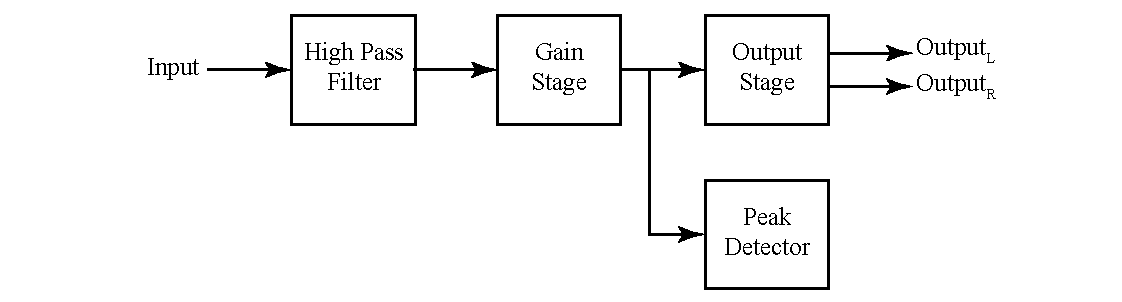
\includegraphics[width=1\textwidth]{Lab10blockdia.pdf}
	\caption{Audio amplifier block diagram. } \label{fig:10blockDia}
\end{figure}

\begin{itemize}
	\item The high pass filter removes the DC offset from the jingle, effectively AC coupling the signal in to the system.
	\item A gain stage is used to amplify the jingle to a range of volts from mV so that it can be heard from the speakers.
	\item An output stage must buffer the output to the speakers, the outputs do not need to be offset in phase.
	\item A peak detector is also required in order to indicate when the output is in the right range, defined by two thresholds. When the output passes the first threshold (LED 1 turns on), the output is operating in the normal linear range with an output on the order of Volts, and the second threshold (LED 2 turns on), where the output is about to start clipping. See the different LED states in \hyperref[tbl:10peakStates]{Table \ref*{tbl:10peakStates}}. Note that this is a slight variation on the circuit used in the diode lab. 
\end{itemize}


\begin{table}
	\centering
\begin{tabular}{| l | l | l |}
	\hline
	\textbf{State} & \textbf{LED 1} & \textbf{LED 2} \\ \hline
	Input < Threshold 1 and 2 & Off & Off \\ \hline
	Threshold 1 < Input < Threshold 2 & On & Off \\ \hline
	Threshold 1 and 2 < Input & On & On \\ \hline
\end{tabular}
	\caption{Different states for the peak detector}
	\label{tbl:10peakStates}
\end{table}

%For the purposes of this class, AM modulation is simple the multiplication of two signals, a high frequency carrier, and a low frequency signal that contains the desired information. The nature of AM modulation results in the low frequency signal forming the envelope of the combined multiplication of the two signals which can be easily extracted using a simple half wave rectifier. 
%
%Unlike a typical AM radio receiver, the input for this circuit will be fixed to the following Wavegen settings, choose \textbf{Modulation} in place of \textbf{Simple} from the pulldown:
%
%\begin{table}[h]
%\begin{center}
%\begin{tabular}{|l|l|l|}
	%\hline
	 %& \textbf{Carrier} & \textbf{Source (AM)} \\ \hline
	%\textbf{Type} & Sine & Sine \\ \hline
	%\textbf{Frequency} & 1.5 MHz & 5 kHz \\ \hline
	%\textbf{Amplitude} / Index: & 1 V & 5\% \\ \hline
	%\textbf{Offset} & 0 V & 0\% \\ \hline
	%\textbf{Symmetry} & 50\% & 50\% \\ \hline
	%\textbf{Phase}: & 0$\deg$ & 0$\deg$ \\ \hline
%\end{tabular}
%\end{center}
%\caption{Wavegen AM modulation settings.}
%\label{tbl:AMwavegen}
%\end{table}
%
%Most of the components have been discussed in previous labs, save for the output stage, and it is up to the student to implement each stage. Beware that there are limited components in your kit, choose your values wisely. A quad op amp chip will also be provided, claim it at office hours or during your lab session.

%%%%%%%%%%%%%%%%%%%%%%%%%%%%%%%%%%%%%%%%%%%%%%%%%%%%%%%%%%%%%%%%%%%%%%%%%%%%%%%%%%%%%%%%%%%%%%%%%%%%%%%
\subsection{Recommendations}
%%%%%%%%%%%%%%%%%%%%%%%%%%%%%%%%%%%%%%%%%%%%%%%%%%%%%%%%%%%%%%%%%%%%%%%%%%%%%%%%%%%%%%%%%%%%%%%%%%%%%%%

\noindent A few words on some of the individual sections. 

\begin{itemize}
	\item As always, you're limited to the components in your lab kit, not the Digilent student kit, choose your values wisely.
	\item Choose the 3dB frequency of the high pass filter carefully. The audio band is 20 Hz to 20 kHz and a 3 dB frequency in the kHz will attenuate (weaken/shrink) important parts of the jingle. Good rule of thumb is if you are over 1 KHz then you are too high. However don't choose it too low, aim for higher than 50 Hz.
	\item The required gain is high, and amplification should occur in two stages. One stage will have a fixed gain. This will be your active high pass filter, both accomplishing the needed filtering and providing gain. The next stage will be another amplifer with variable gain (using a potentiometer as the input resistor). This will allow for a variable voltage on the output signal.
	\item The output stage should be trivial.
	\item Choose the voltage thresholds for the peak detector so that at a reasonable gain, one LED is always on and the other only turns on when the output starts, or is about to start, to clip or distort. 
	\item Use of the active high pass filter for your first stage eliminates the loading effect.
	\item The circuit should pass a demo using sine wave (10mV amplitude, 1KHz, 0,5V DC offset) as input and the peak detection circuit's Threshold 1 and Threshold 2 voltages should be 1V and 4V.  Both LED should be off when the input is <1V, one LED on when the input is between 1V and 4V for OPAMP's linear range operation, then both LEDs should be on when the input is >4V to indicate OPAMP's output is getting into saturation range. The comparator's input configuration is different than Lab 8's, don't copy it directly.
	\item Output stage should have two buffers (for channels L and R).
	\item After you finish the demo and verification of your final project circuits, you need to continue to perform more measurement using scope, spectrum analyzer and network analyzer functions. Follow the file "Final Project Write Up Template" to complete your final report. 
	\item Due time for the final report will be announced in Canvas.  

\end{itemize}

\noindent And some more general advice.

\begin{itemize}
	\item Build everything in LTspice before doing any work on a breadboard. 
	\item The spice simulation of the 19 second jingle file will take a long time, several minutes. The 4 second jingle will also take a few minutes. Start instead with a 10 mV amplitude 1k Hz sine wave with a 0.5 V DC offset and a transient simulation of 1m (.tran 1m). Once you have that working, start using the jingle files. 
	\item Use virtual net nodes instead of making various +5 V and -5 V supplies. 
	\item All of the active components are powered by +5 V and -5 V supplies.
	\item When it's time to build the circuit on a breadboard, build the circuit in a linear fashion. The input should start at one end with the output at the other, don't make it a maze.
	\item Use color coded wires to make debugging easier and avoid creating extra nodes whenever possible. The more nodes in the circuit, the less likely it's going to work.
	\item Build stages one at a time to confirm that they're working as opposed to building everything at once and then trying to debug everything at once. 
	\item Complete the project in the first week, there's a test the second week and it's better to simply get the project out of the way. During the second week you will also need to make time to solder the parts from the project on to a provided PCB for the final demo.
	\item Once you've demoed your circuit, don't take it apart, you'll still need it for items in the write up. It is recommended to complete all measurements required by the write up before soldering to the PCB.
\end{itemize}

%%%%%%%%%%%%%%%%%%%%%%%%%%%%%%%%%%%%%%%%%%%%%%%%%%%%%%%%%%%%%%%%%%%%%%%%%%%%%%%%%%%%%%%%%%%%%%%%%%%%%%%
\section{Pre-Lab Requirements}
%%%%%%%%%%%%%%%%%%%%%%%%%%%%%%%%%%%%%%%%%%%%%%%%%%%%%%%%%%%%%%%%%%%%%%%%%%%%%%%%%%%%%%%%%%%%%%%%%%%%%%%

This following must be completed and submitted to Canvas by the start of lab.

\begin{enumerate}
	\item Image of the spice schematic and a plot of the input and all subsequent outputs (outputs of each individual stage) for a transient simulation for Jingle19 submitted to Canvas. Include the plot of the output and a circuit schematic, nothing else. The schematic and plot should be appropriately labeled. Images that are unclear or vague will receive little to no points. Your plot must include the following in \textbf{different plot planes}: input voltage, output of the high pass filter, output of the variable gain amplifier, output of the buffer stage (at least one), and the current of both LEDs. The gain doesn't need to be high enough to induce clipping in order to show that both LEDs turn on but the first LED should turn on. 
\end{enumerate}

%%%%%%%%%%%%%%%%%%%%%%%%%%%%%%%%%%%%%%%%%%%%%%%%%%%%%%%%%%%%%%%%%%%%%%%%%%%%%%%%%%%%%%%%%%%%%%%%%%%%%%%
\section{In-Lab Requirements}
%%%%%%%%%%%%%%%%%%%%%%%%%%%%%%%%%%%%%%%%%%%%%%%%%%%%%%%%%%%%%%%%%%%%%%%%%%%%%%%%%%%%%%%%%%%%%%%%%%%%%%%

Unlike previous labs, the final project lab spans two weeks (two lab sessions). The final project in-lab portion is only complete once a student has demoed a working circuit. There are two steps to demonstration that a circuit is working:

\begin{enumerate}
	\item Using an input of a 10 mV amplitude sine wave with a 0.5 V DC offset, demonstrate that that the output can be varied and the peak detectors functions properly.
	\item Using the 19 second jingle file as an input, demonstrate that the output can be heard on both speakers and the peak detector functions properly. 
\end{enumerate}

A student can demonstrate their working circuit during either of the two lab sessions, but only in their lab session, not during another lab session or office hours. There are a limited number of connectors and speakers, they will only be handed out to a student once they have demonstrated the first step of the required demonstration.

%%%%%%%%%%%%%%%%%%%%%%%%%%%%%%%%%%%%%%%%%%%%%%%%%%%%%%%%%%%%%%%%%%%%%%%%%%%%%%%%%%%%%%%%%%%%%%%%%%%%%%%
\subsection{Wavegen Settings and Speakers}
%%%%%%%%%%%%%%%%%%%%%%%%%%%%%%%%%%%%%%%%%%%%%%%%%%%%%%%%%%%%%%%%%%%%%%%%%%%%%%%%%%%%%%%%%%%%%%%%%%%%%%%

In order to play the sound file, Jingle19.wav, it must be imported in to the Wavegen's player. Instead of simple, choose play from the pulldown. Click import and then select the Jingle19.wav file. You'll be given a list of options and a plot of the signal, leave the settings to their default and select ok. Hit run to start the jingle playing. 

The 3.5mm connector has three right angle pins soldered to it which allow it to be used with a breadboard. The center pin is ground and the other two pins connect to a speaker. Because the outputs are simply buffered, there's no need for a distinction between left and right. 


%%%%%%%%%%%%%%%%%%%%%%%%%%%%%%%%%%%%%%%%%%%%%%%%%%%%%%%%%%%%%%%%%%%%%%%%%%%%%%%%%%%%%%%%%%%%%%%%%%%%%%%%
%\subsection{Demonstration}
%%%%%%%%%%%%%%%%%%%%%%%%%%%%%%%%%%%%%%%%%%%%%%%%%%%%%%%%%%%%%%%%%%%%%%%%%%%%%%%%%%%%%%%%%%%%%%%%%%%%%%%%
%
%The lab demo consists of the following. Under all conditions, the speaker gain (the volume knob) should be kept to a minimum.
%
%\begin{enumerate}
	%\item Operating of the circuit under normal conditions with the speakers connected. The jingle should be audible on both speakers and the normal LED, case one, should be illuminated. 
	%\item From the previous configuration, the gain is changed in order to induce clipping, which is audible, and should illuminate the other LED, case two. .
%\end{enumerate}

%%%%%%%%%%%%%%%%%%%%%%%%%%%%%%%%%%%%%%%%%%%%%%%%%%%%%%%%%%%%%%%%%%%%%%%%%%%%%%%%%%%%%%%%%%%%%%%%%%%%%%%
\section{Write Up}
%%%%%%%%%%%%%%%%%%%%%%%%%%%%%%%%%%%%%%%%%%%%%%%%%%%%%%%%%%%%%%%%%%%%%%%%%%%%%%%%%%%%%%%%%%%%%%%%%%%%%%%

The write up is also different for the lab project, it takes the form of a formal report. See the template for details. The write up due time will be posted to Canvas, and is typically due around the end of the semester. 









